
Figure \ref{pipeline} summarizes the general methodology that will be discussed. We will focus
on three main components, Data collection, Data processing, and Data exploration.

\ \\ 
\noindent
\begin{tabular}{@{}cc}
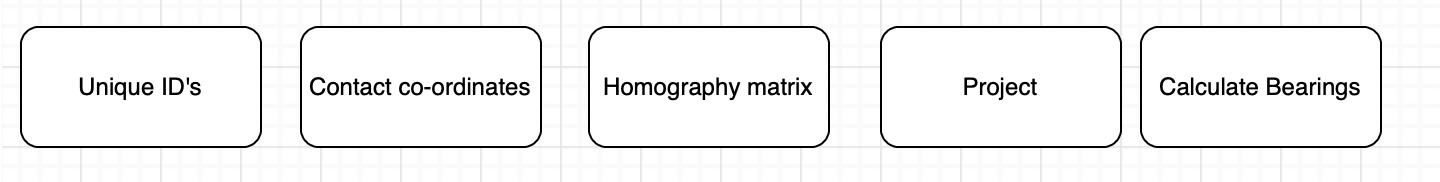
\includegraphics[width=1.0\columnwidth]{temp.png} 
\end{tabular}
\captionof{figure}{Data pipeline overview} 
\label{pipeline}

\subsection{Data Collection}

The Dybbølsbro intersection in Copenhagen was chosen as the location for our primary data collection. 
This intersection faces several challenges producing “conflicts, unsafe situations, illegal road user behavior and great dissatisfaction among road users at the intersection” \cite{CPHpost_2021}.
These challenges make the Dybbølsbro intersection one of the more complicated intersections in Copenhagen and would serve as an excellent base for this quantitative analysis method. 
As this is a large intersection, we have implemented a two cameras recording setup on the opposite side of the intersection; this provides good coverage regardless of traffic obstructions.
\subsubsection{Recording Location}

There are two considerations to take into account when applying these methods to an intersection.
\begin{itemize}
\item intersection size
\end{itemize}
The size of the intersection will determin the camera setup needed. Larger intersections would require a two-camera setup as detailed, but this might not be optimal for intersections much Larger
than the Dybbølsbro intersection. A larger intersection might require more cameras which will need some implementation tweaks. Initially we used a single camera setup, but found that
while we had a good view of the entire intersection we lost a lot of tracking data when cyclist on the opposite side on the intersection where obstructed by vehicles.
\begin{itemize}
\item Camera mounting points
\end{itemize}
We tried four different mounting locations as seen in figure x. The main problems we encountered with these were: Camera stability, obstructions to the camera view, and the height of the mounting positions. Camera stability is partially a mounting system issue, but location x was a bit windy, this caused the camera system to sway a lot more than it would otherwise.
Location Edi and S7 both had a good view of the intersection except for poles blocking part of the view. As location G6 had a good clear view of the intersection and we decided on a two-camera setup
we continued with the recording location S7 as the G6 and S7 combined covered opposing sides of the intersection.


\subsubsection{Camera Selection}

Any camera device with a wide enough field-of-view (FOV) to image the selected intersection, can record at 720p (1280×720 resolution, or 1-megapixel), and that allows remote viewing of its interface,
will suffice however having tested a Raspberry Pi recording setup (Raspberry Pi, camera external battery bank, and an LCD screen case) we would not recommend a setup with self-built recording hardware.
Although the Raspberry Pi setup meets the basic requirements mentioned earlier, the major issue is the usability of such a setup. There are unneeded complexities in
setting up the hardware and having surety of its correct functioning when compared to alternatives that are built and optimized for video recordings such as
mobile phones or action cameras. Mobile phones and action cameras often offer methods of remote viewing of their interfaces that are much more
intuitive than what can be reasonably achieved with a Raspberry Pi setup, as these devices often have data connectivity and/or WIFI allowing for the use of remote control/viewing apps such as TeamViewer.
Being able to remotely view the camera interface is important when mounting the camera and adjusting its position to get a good view of the intersection.

\ \\
For these reasons, we chose to use two mobile phones an LG G6 and a Samsung S7 Edge. Along with meeting the basic requirements they also have Ingress Protection ratings, 
commonly referred to as waterproofing. This should be considered if rain is a possibility.
\ \\

Given a recording location, we can use \ref{eq:1} to calculate the FOV a camera needs to image an intersection.
If $\theta > FOV$, then the FOV is too small.
\color{red}
Note: Label images and make them more understandable.
\color{black}

\begin{equation}
    \theta = tan^-1(\frac{\frac{width}{2}}{adjacent}) * 2\label{eq:1}
  \end{equation}

\ \\ 
\begin{figure}[h]
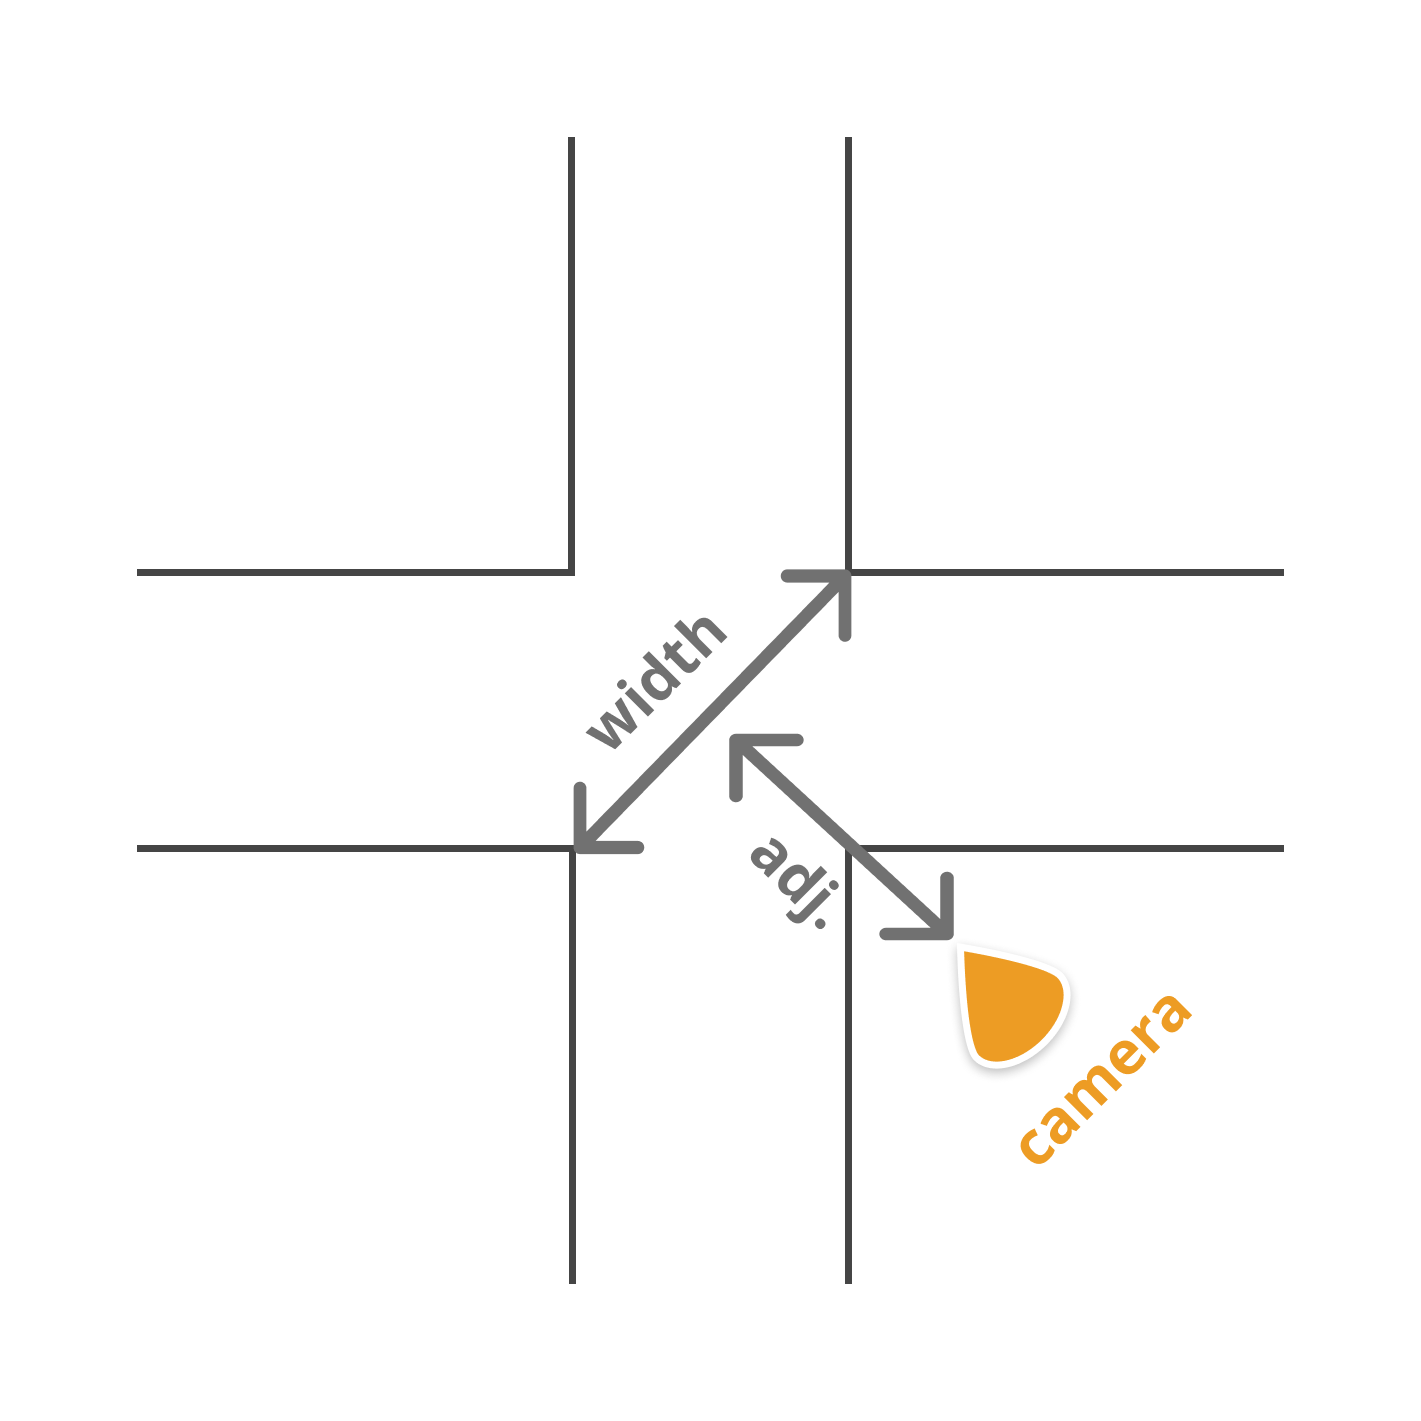
\includegraphics[scale=1.0]{location.png}
\centering 
\end{figure}
\captionof{figure}{Camera location}
\label{Camera location}

\ \\
Battery life and storage capacity should also be considered depending on the amount of intended recording. 
With regards to storage, a good estimate for video size would be 149MB per 1 min of FullHD (1920*1080) at 30FPS. Storage should be selected
with the intended amount of recording time.

\subsubsection{Camera mounting}

As we chose mobile phones to record with we had access to a wide variety of mobile phone mounts on store such as Amazon.
To mount the Samsung S7 Edge we used a flexible arm mount and for the LG G6, we used a custom-made mounting system.
The method of mounting a camera is very much dependant on where the camera is placed and on what. For example, the Samsung S7 Edge's
mounting location was easily accessible and therefore we could simply clamp the system onto a pole. Whereas the LG G6's location was relatively high off the ground and unreachable, therefore we created a mount that allowed us to use an extendable arm to hook the camera onto the position.

For best results, the cameras should be set up as a parallel to the road's surface as possible and high up enough not to have the FOV obstructed by obstacles.
A minimum angle of 30° downwards and a minimum height of 2 meters is recommended.

Note: Picture of our locations and mounting system.

\subsection{Data Processing}

\ \\ 
\noindent
\begin{tabular}{@{}cc}
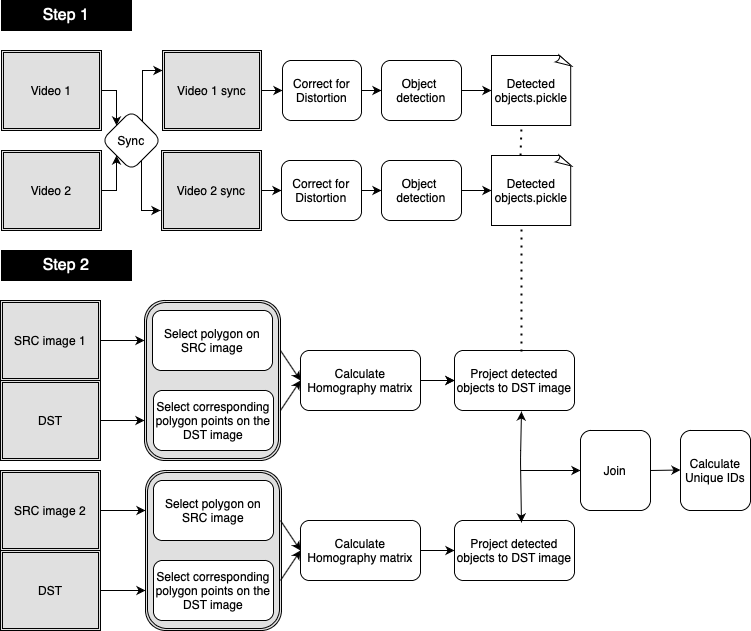
\includegraphics[width=1.0\columnwidth]{data_flow.png} 
\end{tabular}
\captionof{figure}{Data Pipeline}
\label{data}


Figure \ref{data} offers a general overview of the data processing steps. No special hardware is required, but a CUDA-enabled GPU is optimal for object detection using YOLO.
\ \\
\subsubsection{Distortion Correction}

Cameras often suffer from optical aberration where straight lines appear bent. This can be observed on wide-angle camera lenses such as that of the LG G6 used in this study.
The specific type is \textit{positive radial distortion} as shown in figure \ref{distortion}, with lines curving outwards in a barrel shape.
Another form of radial distortion is \textit{pincushion distortion} with lines bend towards the center of the image. These aberrations are a result 
of the curved shape of the camera lens.

Note: Add real examples above.
\ \\ 
\begin{figure}[h]
  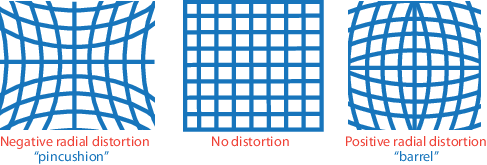
\includegraphics[scale=0.65]{calibration_radial_distortion.png}
  \centering 
  \end{figure}
  \captionof{figure}{Distortion}
  \label{distortion}

\ \\

There is also a possibility of further distortion if the camera sensor and the lens are not parallel, also known as \textit{tangential distortion}.
Ideally, there should be no radial nor tangential distortion.
\ \\
The discovery that leads to the realization that calibration was needed happened in the later stages of constructing this method. When we
started experimenting with joining the video sources did it become evident that distortion was having adverse effects on the data. As we can see in figure 
\ref{joined_distortion} it is clear that the two video sources do not line up.

\begin{figure}[h]
  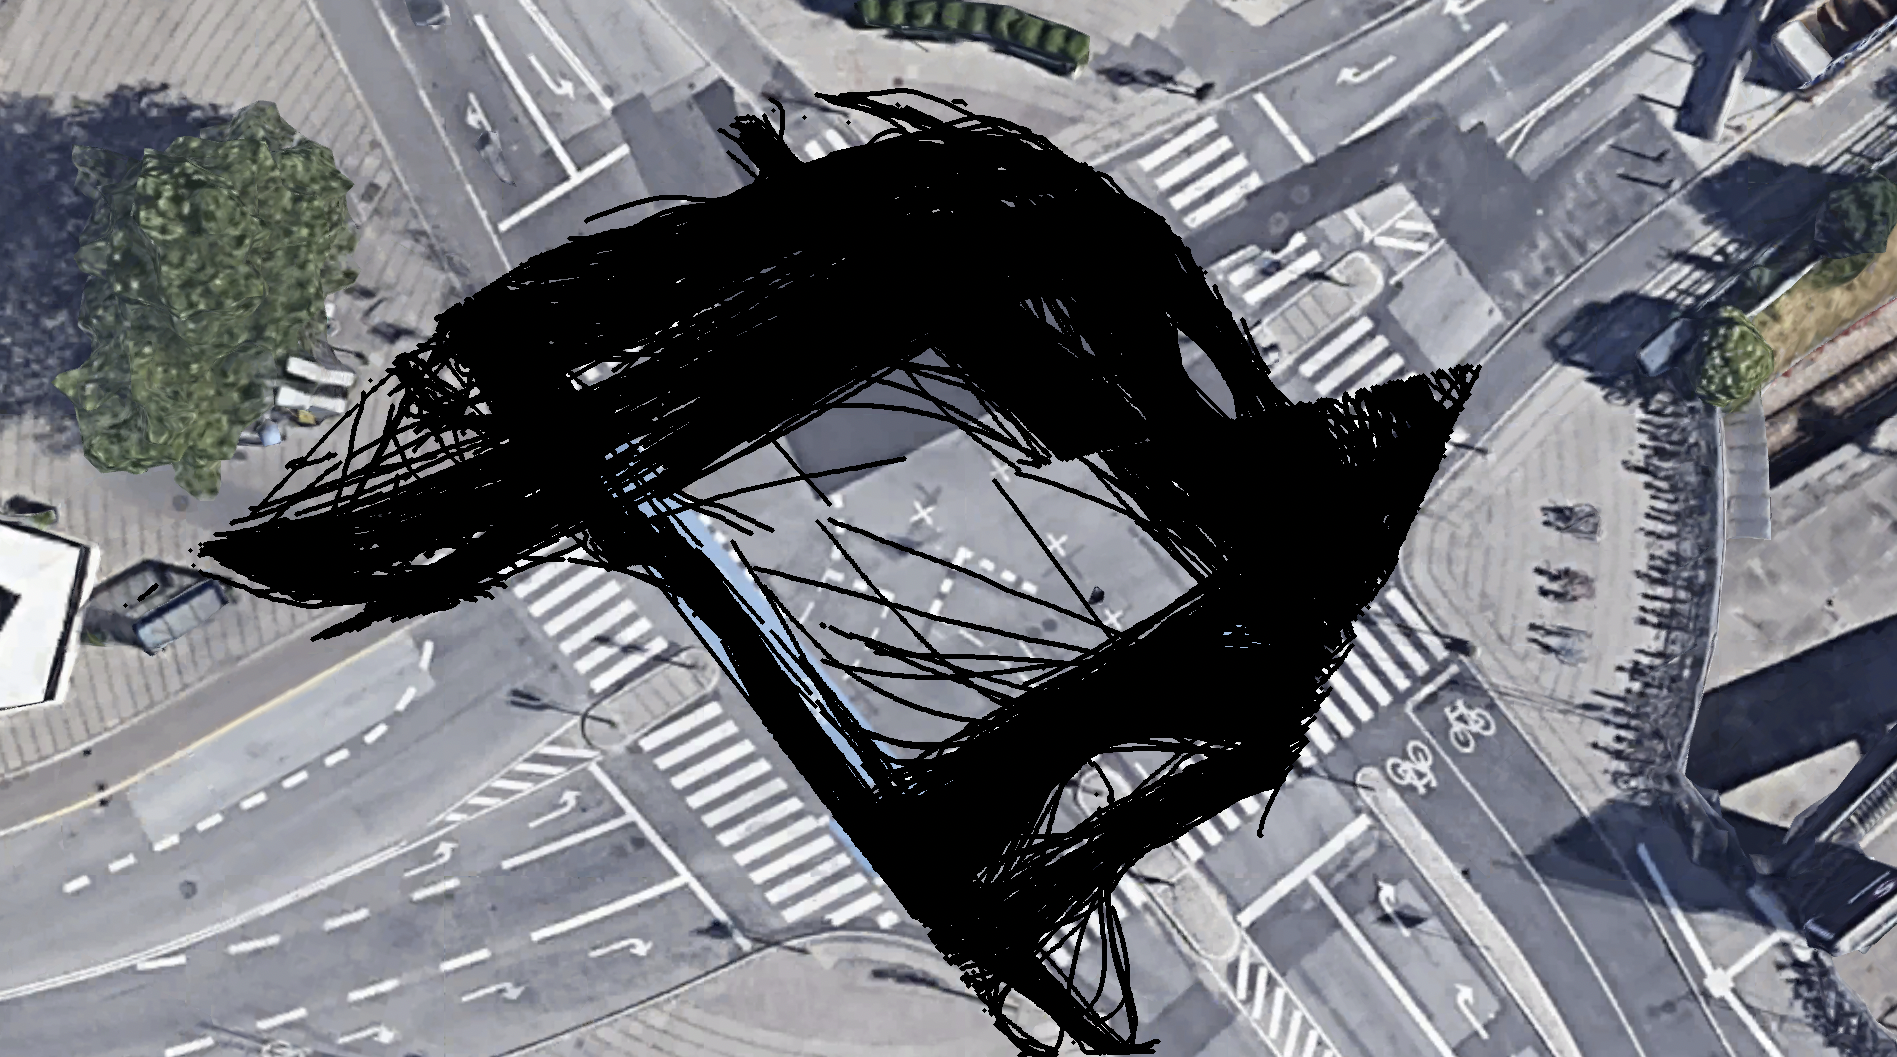
\includegraphics[scale=0.23]{Need_for_calibration.png}
  \centering 
  \end{figure}
  \captionof{figure}{Distortion}
  \label{joined_distortion}
\ \\

In figure \ref{} we can see the results after performing calibration on both video sources and the results are starkly different.

Distortion can lead to incorrect projection and therefore joining of video sources later on.
To correct for this we make use of OpenCVs \cite{noauthor_opencv/opencv_2021} camera calibration toolbox.

In order to correct for distortion, we need to find the camera matrix and distortion coefficients. To do this we used the calibrate.py script provided with OpenCV
passing it several snapshots, taken with the device to be calibrated, of a calibration object as an input. The calibration object being a black-white chessboard pattern.
We passed 20+ sample images of the calibration object in different orientations, angles and positions in the frame. OpenCV processes the calibration object pictures and
return the camera matrix and distortion coefficients.
\ \\
Using the camera matrix and distortion coefficients we then apply OpenCV remap onto each frame in the videos. This unwarps the images.

\ \\
\subsubsection{Object Detection}

Object detection is the most important factor to consider, it is the key component in making this method work. The accuracy of detecting cyclist and the accuracy of the
predicted bounding boxes are the most important data components.
\ \\

We found that our offline OpenDataCam setup using an Nvidia Jetson NX setup worked well for detecting cars but didn't perform well on cyclists. 
We, therefore, implemented our object detection setup using
YOLOv5. YOLOv5 showed a good improvement on cyclists.
\ \\ 
Predicted objects are represented as bounding boxes with the output being represented as $[[frame id][xmin][ymin][xmax][ymax][confidence]]$

\subsubsection{Homography Matrix}

After several failed attempts of trying to analyze the video data in its raw form, we decided a different approach was needed.
These attempts involved trying to interpolate the cardinal direction of each cyclist at specific points in the video. Calculating the cardinal direction
of a cyclist was a matter of adding the cyclist bearing to the cardinal direction of the video frame. The idea being that we could interpret
the desired path by the change in cardinality between 2 or more defined points. These points being selected by where the object detection algorithm worked best.
This however was not a good approach as we would have had to make too many assumptions about the data in addition this was used in conjunction
with OpenDataCam which for our purposes did not produce the desired results.

\ \\
After switching to our own YOLOv5 object detection implementation we decided that we needed to view the data from a different angle and therefore
started exploring the homography matrix.
\ \\
A homography matrix is a transformation matrix between two planes \cite{hartley_zisserman_2004}. It can be used to perform a perspective transformation of a plane from a source image $P(x_r, y_r)$ onto a plane on a destination image $Q(x_i, y_i)$.
The source image in our case is the plane of the road surface from the recorded video at the intersection to the road surface from an aerial view of the same intersection. 
This will allow us to view the cyclist movements from an aerial view.

\ \\ 
\begin{figure}[h]
  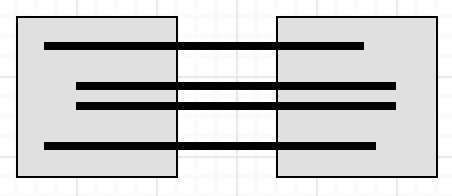
\includegraphics[scale=1.0]{Homography_proj.png}
  \centering 
  \end{figure}
  \captionof{figure}{SR to DST}
  \label{homography}
\ \\ 
To calculate the homography matrix, we need to solve the for the system of linear equations, $P = HQ$,
\ \\
$P$ being points in a polygon on the source image, $Q$ the corresponding polygon on the destination image $H$ being the homography matrix.
\begin{align}
\label{eq:3}
  \begin{bmatrix}
    x_{i} \\
    y_{i} \\
    z_{i} \\
  \end{bmatrix}
  &= \begin{bmatrix}
      h_1 & h_2 & h_3 \\
      h_4 & h_5 & h_6 \\
      h_7 & h_8 & h_9 \\
  \end{bmatrix}
  \begin{bmatrix}
    x_{r} \\
    y_{r} \\
    z_{r} \\
  \end{bmatrix}
\end{align}

\subsubsection{Projection}

Before we can project the cyclist onto an aerial view, we first need to calculate the 2D coordinates of their contact points with the road surface.
Given \ref{representation} we can calculate this by the following

$$x = xmin + \frac{(xmax - xmin)}{2}$$
$$y = ymin$$
\
Using the homography matrix, we can now project the contact points $(x, y)$ of the cyclist onto the destination
image. This is achieved by applying $z$ to each point as a constant to create $Q(x_i, y_i, 1)$ and then we multiply it by the homography matrix. 

\subsubsection{Merging Sources}

To merge the data from the two video sources, we take a naive approach. For optimal coverage, the cameras are set up on
opposite sides of the intersection. We simply cut the video sources in half along the mid-point between
the two cameras along the intersection to join them. The data is then merged.

Example:

\subsubsection{Multiple object tracking}

In order to connect observations into trajectories of individual cyclist, we apply 
simple online and real-time tracking algorithm, SORT \cite{abewley_abewley/sort_2021}, as initially described in \cite{Bewley2016_sort}. 
SORT aims to address multiple object tracking (MOT) where object across frames needs to be connected. 
\color{red}
Note: Explain more about SORT predict bbox then IOU for actualy bbox.
\color{black}
\ \\
We assume arbitrary bounding box dimensions of 10*10 pixels for the projected cyclists to join the tracks from multiple sources. 
Passing the algorithm the bounding boxes per frame, we get a unique ID associated with each observation.

\subsection{Data Exploration}

There are two objectives for the data exploration, those being:
\begin{itemize}
	\item Desire path discovery
	\item Alert Zones - For behaviour observations and counts
\end{itemize}

\subsubsection{Rainbow Tracks}

A method of desire path discovery.

\ \\ 
\noindent
\begin{tabular}{@{}cc}
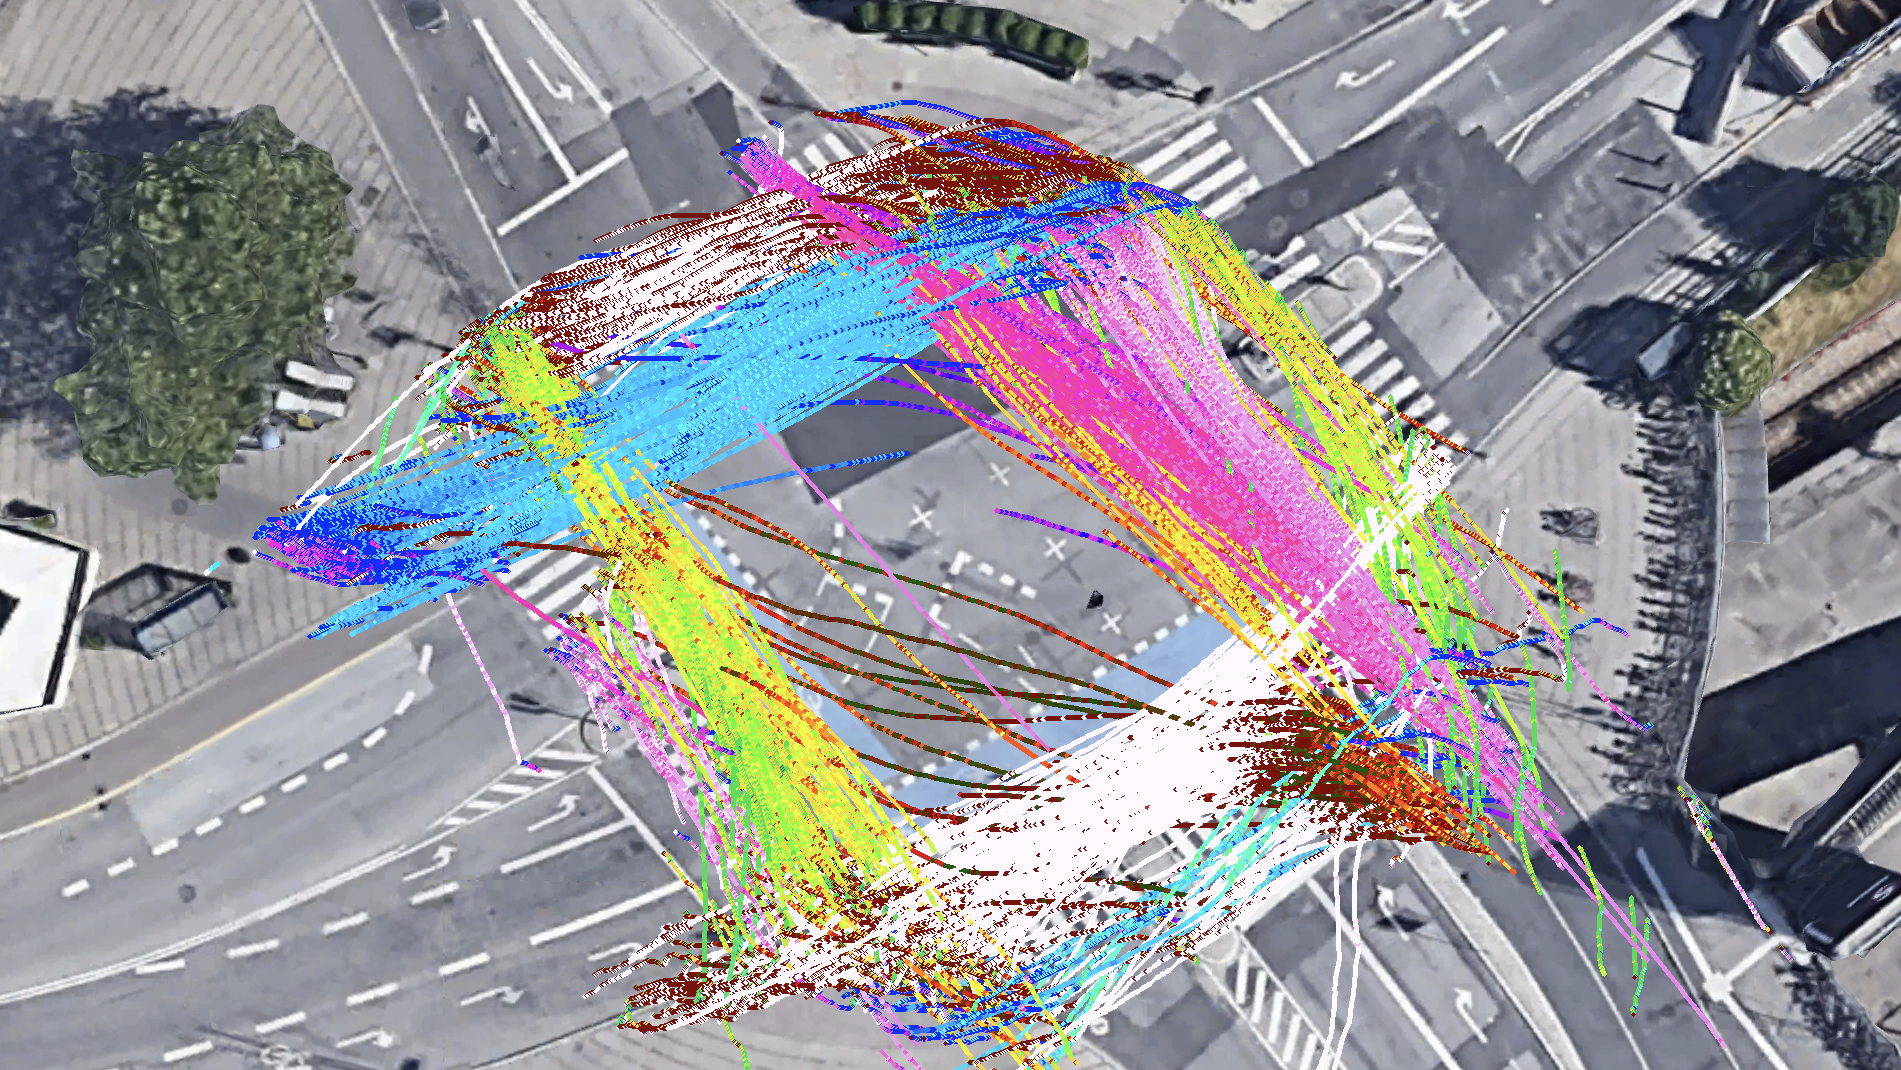
\includegraphics[width=1.0\columnwidth]{rainbow.png} 
\end{tabular}
\captionof{figure}{Rainbow}
\label{Rainbow}
\ \\

To find aggregated desire lines from the data we took an approach which we call "Rainbow tracks". This involves coloring tracks by the bearing between consecutive points in each trajectory. After calculating the bearing, we then get a color from a gradient color wheel. This approach has the added benefit of encoding direction into 
each track.
Note: Maybe just an equation demonstrating the bearing calculation.
\ \\ 

\begin{equation}
  UniqueID_i = [(x_1, y_1)...(x_a+1, y_a+1)]\label{eq:3}
\end{equation}

\subsection{Recognizing abnormal behaviour}

One of
\subsubsection{Deviation from desire lines}
Automatic aproach


\color{red}
We created a "Tool name" that allows the definition of specific areas as "red zones". These zones provide us with easy reference to activity in the zones throughout the videos.
Using these zones, we can count cyclist and observe their behavior at points on the intersection that might be difficult or
problematic.

\subsection{Recognizing abnormal behaviour}

Note: Picture of interface?
